\section*{Exercises}

\begin{ex}
  Consider the following augmented matrix in which $\ast $ denotes an
  arbitrary number and $\blacksquare $ denotes a non-zero number. Determine
  whether the given augmented matrix is consistent. If consistent, is the
  solution unique?
  \begin{equation*}
    \begin{mymatrix}{ccccc|c}
      \blacksquare & \ast & \ast & \ast & \ast & \ast \\
      0 & \blacksquare & \ast & \ast & 0 & \ast \\
      0 & 0 & \blacksquare & \ast & \ast & \ast \\
      0 & 0 & 0 & 0 & \blacksquare & \ast
    \end{mymatrix}
  \end{equation*}
  \begin{sol}
    The solution exists but is not unique.
  \end{sol}
\end{ex}

\begin{ex}
  Consider the following augmented matrix in which $\ast $ denotes an arbitrary
  number and $\blacksquare $ denotes a non-zero number. Determine whether the
  given augmented matrix is consistent. If consistent, is the solution unique?
  \begin{equation*}
    \begin{mymatrix}{ccc|c}
      \blacksquare & \ast & \ast & \ast \\
      0 & \blacksquare & \ast & \ast \\
      0 & 0 & \blacksquare & \ast
    \end{mymatrix}
  \end{equation*}
  \begin{sol}
    A solution exists and is unique.
  \end{sol}
\end{ex}

\begin{ex}
  Consider the following augmented matrix in which $\ast $ denotes an arbitrary
  number and $\blacksquare $ denotes a non-zero number. Determine whether the
  given augmented matrix is consistent. If consistent, is the solution unique?
  \begin{equation*}
    \begin{mymatrix}{ccccc|c}
      \blacksquare & \ast & \ast & \ast & \ast & \ast \\
      0 & \blacksquare & 0 & \ast & 0 & \ast \\
      0 & 0 & 0 & \blacksquare & \ast & \ast \\
      0 & 0 & 0 & 0 & \blacksquare & \ast
    \end{mymatrix}
  \end{equation*}
  % \begin{sol}
  % \end{sol}
\end{ex}

\begin{ex}
  Consider the following augmented matrix in which $\ast $ denotes an arbitrary
  number and $\blacksquare $ denotes a non-zero number. Determine whether the
  given augmented matrix is consistent. If consistent, is the solution unique?
  \begin{equation*}
    \begin{mymatrix}{ccccc|c}
      \blacksquare & \ast & \ast & \ast & \ast & \ast \\
      0 & \blacksquare & \ast & \ast & 0 & \ast \\
      0 & 0 & 0 & 0 & \blacksquare & 0 \\
      0 & 0 & 0 & 0 & \ast & \blacksquare
    \end{mymatrix}
  \end{equation*}
  \begin{sol}
    There might be a solution. If so, there are infinitely many.
  \end{sol}
\end{ex}

\begin{ex}
  Suppose a system of equations has fewer equations than variables. Will such a system necessarily be consistent? If so, explain why and if not, give an example
  which is not consistent.
  \begin{sol}
    No. Consider $x+y+z=2$ and $x+y+z=1$.
  \end{sol}
\end{ex}

\begin{ex}
  If a system of equations has more equations than variables, can it
  have a solution? If so, give an example and if not, explain why not.
  \begin{sol}
    These can
    have a solution. For example, $x+y=1,2x+2y=2,3x+3y=3$ even has an infinite
    set of solutions.
  \end{sol}
\end{ex}

\begin{ex}
  Find $h$ such that
  \begin{equation*}
    \begin{mymatrix}{rr|r}
      2 & h & 4 \\
      3 & 6 & 7
    \end{mymatrix}
  \end{equation*}
  is the augmented matrix of an \textit{inconsistent} system.
  \begin{sol}
    $h=4$
  \end{sol}
\end{ex}

\begin{ex}
  Find $h$ such that
  \begin{equation*}
    \begin{mymatrix}{rr|r}
      1 & h & 3 \\
      2 & 4 & 6
    \end{mymatrix}
  \end{equation*}
  is the augmented matrix of a \textit{consistent} system.
  \begin{sol}
    Any $h$ will work.
  \end{sol}
\end{ex}

\begin{ex}
  Find $h$ such that
  \begin{equation*}
    \begin{mymatrix}{rr|r}
      1 & 1 & 4 \\
      3 & h & 12
    \end{mymatrix}
  \end{equation*}
  is the augmented matrix of a \textit{consistent} system.
  \begin{sol}
    Any $h$ will work.
  \end{sol}
\end{ex}

\begin{ex}
  Choose $h$ and $k$ such that the augmented matrix shown has each of the following:
  \begin{enumerate}
  \item one solution
  \item no solution
  \item infinitely many solutions
  \end{enumerate}
  \begin{equation*}
    \begin{mymatrix}{rr|r}
      1 & h & 2 \\
      2 & 4 & k
    \end{mymatrix}
  \end{equation*}
  \begin{sol}
    If $h\neq 2$ there will be a unique solution for any $k$. If $h=2$ and $%
    k\neq 4$, there are no solutions. If $h=2$ and $k=4$, then there are
    infinitely many solutions.
  \end{sol}
\end{ex}

\begin{ex}
  Choose $h$ and $k$ such that the augmented matrix shown has each of the following:
  \begin{enumerate}
  \item one solution
  \item no solution
  \item infinitely many solutions
  \end{enumerate}
  \begin{equation*}
    \begin{mymatrix}{rr|r}
      1 & 2 & 2 \\
      2 & h & k
    \end{mymatrix}
  \end{equation*}
  \begin{sol}
    If $h\neq 4$, then there is exactly one solution. If $h=4$ and $k\neq 4$,
    then there are no solutions. If $h=4$ and $k=4$, then there are infinitely
    many solutions.
  \end{sol}
\end{ex}

\begin{ex}
  Determine if the system is consistent. If so, is the solution unique?
  \begin{equation*}
    \begin{array}{c}
      x+2y+z-w=2 \\
      x-y+z+w=1 \\
      2x+y-z=1 \\
      4x+2y+z=5
    \end{array}
  \end{equation*}
  \begin{sol}
    There is no solution. The system is inconsistent. You can see this from the
    augmented matrix. $\begin{mymatrix}{rrrr|r}
      1 & 2 & 1 & -1 & 2 \\
      1 & -1 & 1 & 1 & 1 \\
      2 & 1 & -1 & 0 & 1 \\
      4 & 2 & 1 & 0 & 5
    \end{mymatrix}$, {\ef}: $\begin{mymatrix}{rrrr|r}
      1 & 2 & 1 & -1 & 2 \\
      0 & -3 & 0 & 2 & -1 \\
      0 & 0 & -3 & 0 & -2 \\
      0 & 0 & 0 & 0 & 1
    \end{mymatrix}$.
  \end{sol}
\end{ex}

\begin{ex}
  Determine if the system is consistent. If so, is the solution unique?
  \begin{equation*}
    \begin{array}{c}
      x+2y+z-w=2 \\
      x-y+z+w=0 \\
      2x+y-z=1 \\
      4x+2y+z=3
    \end{array}
  \end{equation*}
  \begin{sol}
    Solution is: $\mat{w=\frac{3}{2}y-1,x=\frac{2}{3}-\frac{1}{2}y,z=\frac{1}{3
      }} $
  \end{sol}
\end{ex}

\begin{ex}
  Determine which matrices are in {\ef}.
  \begin{equation*}
    (a)~
    \begin{mymatrix}{rrrr}
      1 & 1 & 2 & 0 \\
      0 & 0 & 3 & 2 \\
      0 & 0 & 0 & 0
    \end{mymatrix}
    \quad
    (b)~
    \begin{mymatrix}{rrr}
      1 & 0 & 0 \\
      2 & 1 & 7
    \end{mymatrix}
    \quad
    (c)~
    \begin{mymatrix}{rrrrrr}
      0 & 1 & 0 & 0 & 5 \\
      0 & 0 & 1 & 0 & 4 \\
      0 & 0 & 0 & 1 & 3
    \end{mymatrix}
  \end{equation*}
  \begin{sol}
    (a) Yes. (b) No. (c) Yes.
  \end{sol}
\end{ex}

\begin{ex}\label{ex:rr-ef}
  Row reduce each of the following matrices to {\ef}.
  \begin{equation*}
    (a)~
    \begin{mymatrix}{rrrr}
      2 & -1 & 3 & -1 \\
      1 & 0 & 2 & 1 \\
      1 & -1 & 1 & -2
    \end{mymatrix}
    \quad
    (b)~
    \begin{mymatrix}{rrrr}
      0 & 0 & -1 & -1 \\
      1 & 1 & 1 & 0 \\
      1 & 1 & 0 & -1
    \end{mymatrix}
    \quad
    (c)~
    \begin{mymatrix}{rrrr}
      3 & -6 & -7 & -8 \\
      1 & -2 & -2 & -2 \\
      1 & -2 & -3 & -4
    \end{mymatrix}
  \end{equation*}
  \begin{equation*}
    (d)~
    \begin{mymatrix}{rrrr}
      2 & 4 & 5 & 15 \\
      1 & 2 & 3 & 9 \\
      1 & 2 & 2 & 6
    \end{mymatrix}
    \quad
    (e)~
    \begin{mymatrix}{rrrr}
      4 & -1 & 7 & 10 \\
      1 & 0 & 3 & 3 \\
      1 & -1 & -2 & 1
    \end{mymatrix}
    \quad
    (f)~
    \begin{mymatrix}{rrrr}
      3 & 5 & -4 & 2 \\
      1 & 2 & -1 & 1 \\
      1 & 1 & -2 & 0
    \end{mymatrix}
  \end{equation*}
  \begin{equation*}
    (g)~
    \begin{mymatrix}{rrrr}
      -2 & 3 & -8 & 7 \\
      1 & -2 & 5 & -5 \\
      1 & -3 & 7 & -8
    \end{mymatrix}
  \end{equation*}
  % \begin{sol}
  % \end{sol}
\end{ex}

\begin{ex}
  Find the general solution of the system whose augmented matrix is
  \begin{equation*}
    (a)~
    \begin{mymatrix}{rrr|r}
      1 & 2 & 0 & 2 \\
      1 & 3 & 4 & 2 \\
      1 & 0 & 2 & 1
    \end{mymatrix}
    \quad
    (b)~
    \begin{mymatrix}{rrr|r}
      1 & 2 & 0 & 2 \\
      2 & 0 & 1 & 1 \\
      3 & 2 & 1 & 3
    \end{mymatrix}
    \quad
    (c)~
    \begin{mymatrix}{rrr|r}
      1 & 1 & 0 & 1 \\
      1 & 0 & 4 & 2
    \end{mymatrix}
  \end{equation*}
  \begin{equation*}
    (d)~
    \begin{mymatrix}{rrrrr|r}
      1 & 0 & 2 & 1 & 1 & 2 \\
      0 & 1 & 0 & 1 & 2 & 1 \\
      1 & 2 & 0 & 0 & 1 & 3 \\
      1 & 0 & 1 & 0 & 2 & 2
    \end{mymatrix}
    \quad
    (e)~
    \begin{mymatrix}{rrrrr|r}
      1 & 0 & 2 & 1 & 1 & 2 \\
      0 & 1 & 0 & 1 & 2 & 1 \\
      0 & 2 & 0 & 0 & 1 & 3 \\
      1 & -1 & 2 & 2 & 2 & 0
    \end{mymatrix}
  \end{equation*}

  \begin{sol}
    (b) The {\ef} is
    $\def\arraystretch{1.3}
    \begin{mymatrix}{rrr|r}
      1 & 0 & \frac{1}{2} & \frac{1}{2} \\
      0 & 1 & -\frac{1}{4} & \frac{3}{4} \\
      0 & 0 & 0 & 0
    \end{mymatrix}$. Therefore, the solution is of the form $z=t, y=\frac{3}{4}+t\paren{
      \frac{1}{4}}, x=\frac{1}{2}-\frac{1}{2}t$ where $t\in \R$.

    (c) The {\ef} is $\begin{mymatrix}{rrr|r}
      1 & 0 & 4 & 2 \\
      0 & 1 & -4 & -1
    \end{mymatrix} $ and so the solution is $z=t,y=-1+4t,x=2-4t$.

    (d) The {\ef} is $\begin{mymatrix}{rrrrr|r}
      1 & 0 & 0 & 0 & 9 & 3 \\
      0 & 1 & 0 & 0 & -4 & 0 \\
      0 & 0 & 1 & 0 & -7 & -1 \\
      0 & 0 & 0 & 1 & 6 & 1
    \end{mymatrix} $ and so $x_5=t,x_4=1-6t,x_3=-1+7t,x_2=4t,x_1=3-9t$.

    (e) The {\ef} is
    $\def\arraystretch{1.3}
    \begin{mymatrix}{rrrrr|r}
      1 & 0 & 2 & 0 & -\frac{1}{2} & \frac{5}{2} \\
      0 & 1 & 0 & 0 & \frac{1}{2} & \frac{3}{2} \\
      0 & 0 & 0 & 1 & \frac{3}{2} & -\frac{1}{2} \\
      0 & 0 & 0 & 0 & 0 & 0
    \end{mymatrix}$. Therefore, let $x_5=t,x_3=s$. Then the other
    variables are given by
    $x_4=-\frac{1}{2}-\frac{3}{2}t, x_2=\frac{3}{2}-t\frac{1}{2},,
    x_1=\frac{5}{2}+\frac{1}{2}t-2s$.
  \end{sol}
\end{ex}

\begin{ex}
  Solve the system of equations $7x+14y+15z=22,
  $ $2x+4y+3z=5$, and $3x+6y+10z=13$.
  \begin{sol}
    Solution is: $\mat{x=1-2t,z=1,y=t} $
  \end{sol}
\end{ex}

\begin{ex}
  Solve the system of equations $3x-y+4z=6$,
  $y+8z=0$, and $-2x+y=-4$.
  \begin{sol}
    Solution is: $\mat{x=2-4t,y=-8t,z=t} $
  \end{sol}
\end{ex}

\begin{ex}
  Solve the system of equations $9x-2y+4z=-17,
  $ $13x-3y+6z=-25$, and $-2x-z=3$.
  \begin{sol}
    Solution is: $\mat{x=-1,y=2,z=-1} $
  \end{sol}
\end{ex}

\begin{ex}
  Solve the system of equations
  $65x+84y+16z=546$, $81x+105y+20z=682$, and $84x+110y+21z=713$.
  \begin{sol}
    Solution is:
    $\mat{x=2,y=4,z=5} $
  \end{sol}
\end{ex}

\begin{ex}
  Solve the system of equations
  $8x+2y+3z=-3,8x+3y+3z=-1$, and $4x+y+3z=-9$.
  \begin{sol}
    Solution is: $\mat{x=1,y=2,z=-5} $
  \end{sol}
\end{ex}

\begin{ex}
  Suppose a system of equations has fewer equations than variables and
  you have found a solution to this system of equations. Is it possible that
  your solution is the only one?\ Explain.
  \begin{sol}
    No. Consider $x+y+z=2$ and $x+y+z=1$.
  \end{sol}
\end{ex}

\begin{ex}
  Suppose a system of linear equations has an augmented
  matrix with 2 rows and 4 columns and the last column is a pivot
  column. Could the system of linear equations be consistent? Explain.
  \begin{sol}
    No. This would lead to $0=1$.
  \end{sol}
\end{ex}

\begin{ex}
  Suppose the coefficient matrix of a system of $n$ equations with $n$
  variables has the property that every column is a pivot column. Does it
  follow that the system of equations must have a solution? If so, must the
  solution be unique? Explain.
  \begin{sol}
    Yes. It has a unique solution.
  \end{sol}
\end{ex}

\begin{ex}
  Suppose there is a unique solution to a system of linear equations.
  What must be true of the pivot columns in the augmented matrix?
  \begin{sol}
    The last column must not be a pivot column. The remaining columns must each be pivot
    columns.
  \end{sol}
\end{ex}

\begin{ex}
  The steady state temperature, $u$, of a plate solves Laplace's
  equation, $\Delta u=0$. One way to approximate the solution is to divide the plate into a square mesh and require the temperature
  at each node to equal the average of the temperature at the four adjacent
  nodes. In the following picture, the numbers represent the observed
  temperature at the indicated nodes. Find the temperature at
  the interior nodes, indicated by $x,y,z$, and $w$. One of the equations is
  $z=\frac{1}{4}(10+0+w+x)$.

  \begin{center}
    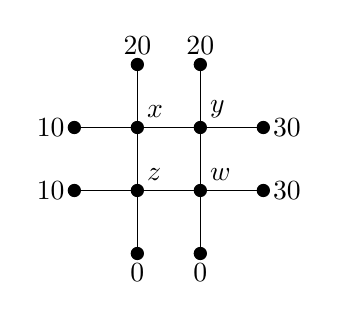
\begin{tikzpicture}[scale=0.8]
      \draw (1,0) -- (1,3);
      \draw (2,0) -- (2,3);
      \draw (0,1) -- (3,1);
      \draw (0,2) -- (3,2);
      \fill (0,1) circle (3pt) node[left]{$10$};
      \fill (0,2) circle (3pt) node[left]{$10$};
      \fill (1,0) circle (3pt) node[below]{$0$};
      \fill (1,1) circle (3pt) node[above right]{$z$};
      \fill (1,2) circle (3pt) node[above right]{$x$};
      \fill (1,3) circle (3pt) node[above]{$20$};
      \fill (2,0) circle (3pt) node[below]{$0$};
      \fill (2,1) circle (3pt) node[above right]{$w$};
      \fill (2,2) circle (3pt) node[above right]{$y$};
      \fill (2,3) circle (3pt) node[above]{$20$};
      \fill (3,1) circle (3pt) node[right]{$30$};
      \fill (3,2) circle (3pt) node[right]{$30$};
    \end{tikzpicture}
  \end{center}
  \begin{sol}
    You need $\def\arraystretch{1.2}
    \begin{array}{r}
      \frac{1}{4}(20+30+w+x) -y=0 \\
      \frac{1}{4}(y+30+0+z) -w=0 \\
      \frac{1}{4}(20+y+z+10) -x=0 \\
      \frac{1}{4}(x+w+0+10) -z=0
    \end{array}
    $. Solution is: $\mat{x=15,y=20,z=10,w=15}$.
  \end{sol}
\end{ex}

\begin{ex}
  Find the rank of the following matrices.
  \begin{equation*}
    (a)~
    \begin{mymatrix}{rrrr}
      4 & -16 & -1 & -5 \\
      1 & -4 & 0 & -1 \\
      1 & -4 & -1 & -2
    \end{mymatrix}
    \quad
    (b)~
    \begin{mymatrix}{rrrr}
      3 & 6 & 5 & 12 \\
      1 & 2 & 2 & 5 \\
      1 & 2 & 1 & 2
    \end{mymatrix}
    \quad
    (c)~
    \begin{mymatrix}{rrrrr}
      0 & 0 & -1 & 0 & 3 \\
      1 & 4 & 1 & 0 & -8 \\
      1 & 4 & 0 & 1 & 2 \\
      -1 & -4 & 0 & -1 & -2
    \end{mymatrix}
  \end{equation*}
  \begin{equation*}
    (d)~
    \begin{mymatrix}{rrrrr}
      1 & -2 & 0 & 3 & 11 \\
      1 & -2 & 0 & 4 & 15 \\
      1 & -2 & 0 & 3 & 11 \\
      0 & 0 & 0 & 0 & 0
    \end{mymatrix}
    \quad
    (e)~
    \begin{mymatrix}{rrr}
      -2 & -3 & -2 \\
      1 & 1 & 1 \\
      1 & 0 & 1 \\
      -3 & 0 & -3
    \end{mymatrix}
  \end{equation*}
  % \begin{sol}
  % \end{sol}
\end{ex}

\begin{ex}
  Suppose $A$ is an $m\times n$-matrix. Explain why the rank of $A$ is
  always no larger than $\min (m,n)$.
  \begin{sol}
    The rank is the number of pivot entries in the {\ef}. There is at
    most one pivot entry in each row and column. Therefore, the rank
    cannot be larger than the number of rows or the number of columns;
    in other words, the rank is at most $\min(m,n)$.
  \end{sol}
\end{ex}

\begin{ex}
  State whether each of the following sets of data is
  possible for a system of equations. If possible, describe the
  solution set.  That is, indicate whether there exists a unique
  solution, no solution or infinitely many solutions. Here, $A$ is
  the coefficient matrix, and $\mat{A\mid B}$ denotes the
  augmented matrix of the system.

  \begin{enumerate}
  \item $A$ is a $5\times 6$-matrix, $\rank(A) =4$ and
    $\rank\mat{A\mid B} =4$.

  \item $A$ is a $3\times 4$-matrix, $\rank(A) =3$ and
    $\rank\mat{A\mid B} =2$.

  \item $A$ is a $4\times 2$-matrix, $\rank(A) =4$ and
    $\rank\mat{A\mid B} =4$.

  \item $A$ is a $5\times 5$-matrix, $\rank(A) =4$ and
    $\rank\mat{A\mid B} =5$.

  \item $A$ is a $4\times 2$-matrix, $\rank(A) =2$ and
    $\rank\mat{A\mid B} =2$.
  \end{enumerate}

  \begin{sol}
    \begin{enumerate}
    \item The {\ef} has 4 non-zero rows and 6 columns, so there are 2
      free variables, and the system has infinitely many solutions.
    \item Such a system of equations of equations does not exist. If
      you add in another column, the rank does not get smaller.
    \item Such a system of equations does not exist,
      because the rank cannot equal 4 if there are only two columns.
    \item The {\ef} has 4 non-zero rows on the left-hand side, but 5
      non-zero rows if we also include the right-hand side. Therefore
      the system is inconsistent, i.e., it has no solutions.
    \item The {\ef} has 2 non-zero rows, so there are 2
      pivot variables and no free variables. Therefore, the system has
      a unique solution.
    \end{enumerate}
  \end{sol}
\end{ex}

\begin{ex}
  Consider the system $-5x+2y-z=0$ and $-5x-2y-z=0$. Both equations
  equal zero and so $-5x+2y-z=-5x-2y-z$ which is equivalent to $y=0$. Does it follow that $x$
  and $z$ can equal anything?  Notice that when $x=1$, $z=-4$, and $y=0$ are plugged in
  to the equations, the equations do not equal $0$. Why?
  \begin{sol}
    These are not legitimate row
    operations. They do not preserve the solution set of the system.
  \end{sol}
\end{ex}
